\documentclass[table]{beamer}
%[]中可以使用draft、handout、screen、transparency、trancompress、compress等参数

%指定beamer的模式与主题
\mode<presentation>
{
  \usetheme{Madrid}
%\usetheme{Boadilla}
%\usecolortheme{default}
%\usecolortheme{orchid}
%\usecolortheme{whale}
%\usefonttheme{professionalfonts}
}

%\usetheme{Madrid}
%这里还可以选择别的主题:Bergen, Boadilla, Madrid, AnnArbor, CambridgeUS, Pittsburgh, Rochester, Warsaw, ...
%有导航栏的Antibes, JuanLesPins, Montpellier, ...
%有内容的Berkeley, PaloAlto, Goettingen, Marburg, Hannover, ...
%有最小导航栏的Berlin, Ilmenau, Dresden, Darmstadt, Frankfurt, Singapore, Szeged, ...
%有章和节表单的Copenhagen, Luebeck, Malmoe, Warsaw, ...

%\usecolortheme{default}
%设置内部颜色主题(这些主题一般改变block里的颜色);这个主题一般选择动物来命名
%这里还可以选择别的颜色主题,如默认的和有特别目的的颜色主题default,structure,sidebartab,全颜色主题albatross,beetle,crane,dove,fly,seagull,wolverine,beaver

%\usecolortheme{orchid}
%设置外部颜色主题(这些主题一般改变title里的颜色);这个主题一般选择植物来命名
%这里还可以选择别的颜色主题,如默认的和有特别目的的颜色主题lily,orchid,rose

%\usecolortheme{whale}
%设置字体主题;这个主题一般选择海洋动物来命名
%这里还可以选择别的颜色主题,如默认的和有特别目的的颜色主题whale,seahorse,dolphin

%\usefonttheme{professionalfonts}
%类似的还可以定义structurebold,structuresmallcapsserif,professionalfonts

% 控制 beamer 的风格,可以根据自己的爱好修改
%\usepackage{beamerthemesplit} %使用 split 风格
%\usepackage{beamerthemeshadow} %使用 shadow 风格
%\usepackage[width=2cm,dark,tab]{beamerthemesidebar}

%插入音标
%\usepackage{tipa}
%\AtBeginDocument{
  %\renewcommand\textipa{\fontencoding{T3}\selectfont}
%}
%\AtBeginDocument{
  %\renewcommand\textipa[2][r]{{\fontfamily{cm#1}\tipaencoding #2}}
%}
%\renewenvironment{IPA}[1][r]
 %{\fontfamily{cm#1}\tipaencoding}
 %{}

% 设定英文字体
%\usepackage{fontspec}
% Fix bugs for fontspec in TeXLive2015
\ifdefined\suppressfontnotfounderror
  \expandafter\let\csname xetex_suppressfontnotfounderror:D\endcsname
    \suppressfontnotfounderror
\else
  \expandafter\let\csname xetex_suppressfontnotfounderror:D\endcsname
    \luatexsuppressfontnotfounderror
\fi
\usepackage[no-math]{fontspec}
\setmainfont{Times New Roman}
\setsansfont{Arial}
\setmonofont{Courier New}

% 设定中文字体
\usepackage[BoldFont,SlantFont,CJKchecksingle,CJKnumber]{xeCJK}
%\setCJKmainfont[BoldFont={Adobe Heiti Std},ItalicFont={Adobe Kaiti Std}]{Adobe Song Std}
\setCJKmainfont[BoldFont={Adobe Heiti Std},ItalicFont={Adobe Kaiti Std}]{WenQuanYi Micro Hei}
\setCJKsansfont{Adobe Heiti Std}
\setCJKmonofont{Adobe Fangsong Std}
\punctstyle{hangmobanjiao}

\defaultfontfeatures{Mapping=tex-text}
\usepackage{xunicode}
\usepackage{xltxtra}

\XeTeXlinebreaklocale "zh"
\XeTeXlinebreakskip = 0pt plus 1pt minus 0.1pt

\usepackage{setspace}
\usepackage{colortbl,xcolor}
\usepackage{hyperref}
%\hypersetup{xetex,bookmarksnumbered=true,bookmarksopen=true,pdfborder=1,breaklinks,colorlinks,linkcolor=blue,filecolor=black,urlcolor=cyan,citecolor=green}
\hypersetup{xetex,bookmarksnumbered=true,bookmarksopen=true,pdfborder=1,breaklinks,colorlinks,linkcolor=cyan,filecolor=black,urlcolor=blue,citecolor=green}

% 插入图片
\usepackage{graphicx}
\graphicspath{{figures/}}
% 图文混排
%\usepackage{picins}
\usepackage{floatflt}

% 可能用到的包
\usepackage{amsmath,amssymb}
%插入多媒体
%\usepackage{media9}
%\usepackage{movie15}
\usepackage{multimedia}
\usepackage{multicol}
\usepackage{multirow}

% 定义一些自选的模板,包括背景、图标、导航条和页脚等,修改要慎重
% 设置背景渐变由10%的红变成10%的结构颜色
%\beamertemplateshadingbackground{red!10}{structure!10}
%\beamertemplatesolidbackgroundcolor{white!90!blue}
% 使所有隐藏的文本完全透明、动态,而且动态的范围很小
\beamertemplatetransparentcovereddynamic
% 使itemize环境中变成小球,这是一种视觉效果
\beamertemplateballitem
% 为所有已编号的部分设置一个章节目录,并且编号显示成小球
\beamertemplatenumberedballsectiontoc
% 将每一页的要素的要素名设成加粗字体
\beamertemplateboldpartpage

% item逐步显示时,使已经出现的item、正在显示的item、将要出现的item呈现不同颜色
\def\hilite<#1>{
 \temporal<#1>{\color{gray}}{\color{blue}}
    {\color{blue!25}}
}

\renewcommand{\today}{\number\year 年 \number\month 月 \number\day 日}

%五角星
\usepackage{MnSymbol}

%去除图表标题中的figure等
\usepackage{caption}
\captionsetup{labelformat=empty,labelsep=none}

\usepackage{tabu}
\usepackage{multirow}
%表格自动换行
\usepackage{tabularx} 

% 千分号
%\usepackage{textcomp}

%罗马数字
\makeatletter
\newcommand{\rmnum}[1]{\romannumeral #1}
\newcommand{\Rmnum}[1]{\expandafter\@slowromancap\romannumeral #1@}
\makeatother

%分栏
\usepackage{multicol}

%\usepackage{enumitem}
%\usepackage{enumerate}

%键盘
\usepackage{keystroke}

%心形
%\usepackage{fdsymbol}

%插入源代码
\usepackage{listings}
\lstset{
  language=perl,                  % 程序语言名称:TeX, Perl, R, sh, bash, Awk
  basicstyle=\normalsize\tt,      %\tt指monospace字体族,程序源代码使用此族字体表示更加美观
  numbers=left,                   % 行号位置(左侧)
  numberstyle=\small,             % 行号字体的字号
  stepnumber=1,                   % 行号的显示步长
  numbersep=5pt,                  % 行号与代码间距
  backgroundcolor=\color{white},  % 背景色;需要 \usepackage{color}
  showspaces=false,               % 不显示空格
  showstringspaces=false,         % 不显示代码字符串中的空格标记
  showtabs=false,                 % 不显示 TAB
  tabsize=4, 
  frame=shadowbox,                % 把代码用带有阴影的框圈起来
  captionpos=b,                   % 标题位置
  breaklines=true,                % 对过长的代码自动断行
  breakatwhitespace=false,        % 断行只在空格处
  extendedchars=false,            % 解决代码跨页时,章节标题,页眉等汉字不显示的问题
  %escapeinside={\%*}{*},         % 跳脱字符,添加注释,暂时离开 listings 
  %escapeinside=``,
  commentstyle=\color{red!50!green!50!blue!50}\tt,  %浅灰色的注释
  rulesepcolor=\color{red!20!green!20!blue!20},     %代码块边框为淡青色
  keywordstyle=\color{blue!70}\bfseries\tt,         %代码关键字的颜色为蓝色,粗体
  identifierstyle=\tt,
  stringstyle=\tt,                % 代码字符串的特殊格式
  keepspaces=true,
  breakindent=1em,
  %breakindent=22pt,
  %breakindent=4em,
  breakautoindent=true,
  flexiblecolumns=true,
  aboveskip=1em,                  %代码块边框
  xleftmargin=2em,
  xrightmargin=2em
}

%\setbeamercolor{alerted text}{fg=magenta}
\setbeamercolor{bgcolor}{fg=yellow,bg=cyan}
%\setbeamercolor{itemize/enumerate body}{fg=green}

\begin{document}

%\includeonlyframes{current}

\logo{
\includegraphics[height=0.08\textwidth]{qr.png}}

% 在每个Section前都会加入的Frame
\AtBeginSection[]
{
  \begin{frame}<beamer>
    %\frametitle{Outline}
    \frametitle{教学提纲}
    \setcounter{tocdepth}{3}
    \begin{multicols}{2}
      \tableofcontents[currentsection,currentsubsection]
      %\tableofcontents[currentsection]
    \end{multicols}
  \end{frame}
}
% 在每个Subsection前都会加入的Frame
\AtBeginSubsection[]
{
  \begin{frame}<beamer>
%%\begin{frame}<handout:0>
%% handout:0 表示只在手稿中出现
    \frametitle{教学提纲}
    \setcounter{tocdepth}{3}
    \begin{multicols}{2}
    \tableofcontents[currentsection,currentsubsection]
    \end{multicols}
%% 显示在目录中加亮的当前章节
  \end{frame}
}

% 为当前幻灯片设置背景
%{
%\usebackgroundtemplate{
%\vbox to \paperheight{\vfil\hbox to
%\paperwidth{\hfil\includegraphics[width=2in]{tijmu_charcoal.png}\hfil}\vfil}
%}
\begin{frame}[plain]
  \begin{center}
    {\Huge 疯狂的实验\\}
    \vspace{1cm}
    {\LARGE 天津医科大学\\}
    %\vspace{0.2cm}
    {\LARGE 生物医学工程与技术学院\\}
    \vspace{1cm}
    {\large 2018-2019学年下学期(春)\\ 公共选修课}
  \end{center}
\end{frame}
%}



%\includeonlyframes{current}

\title[生物学]{第四章\quad 疯狂的实验——生物学}
\author[Yixf]{伊现富(Yi Xianfu)}
\institute[TIJMU]{天津医科大学(TIJMU)\\ 生物医学工程与技术学院}
\date{2019年4月}

\begin{frame}
  \titlepage
\end{frame}

\begin{frame}[plain,label=current]
  \frametitle{教学提纲}
  \setcounter{tocdepth}{3}
  \begin{multicols}{2}
    \tableofcontents
  \end{multicols}
\end{frame}


\section{生物钟}
\begin{frame}
  \frametitle{生物钟}
  \begin{figure}
    \centering
    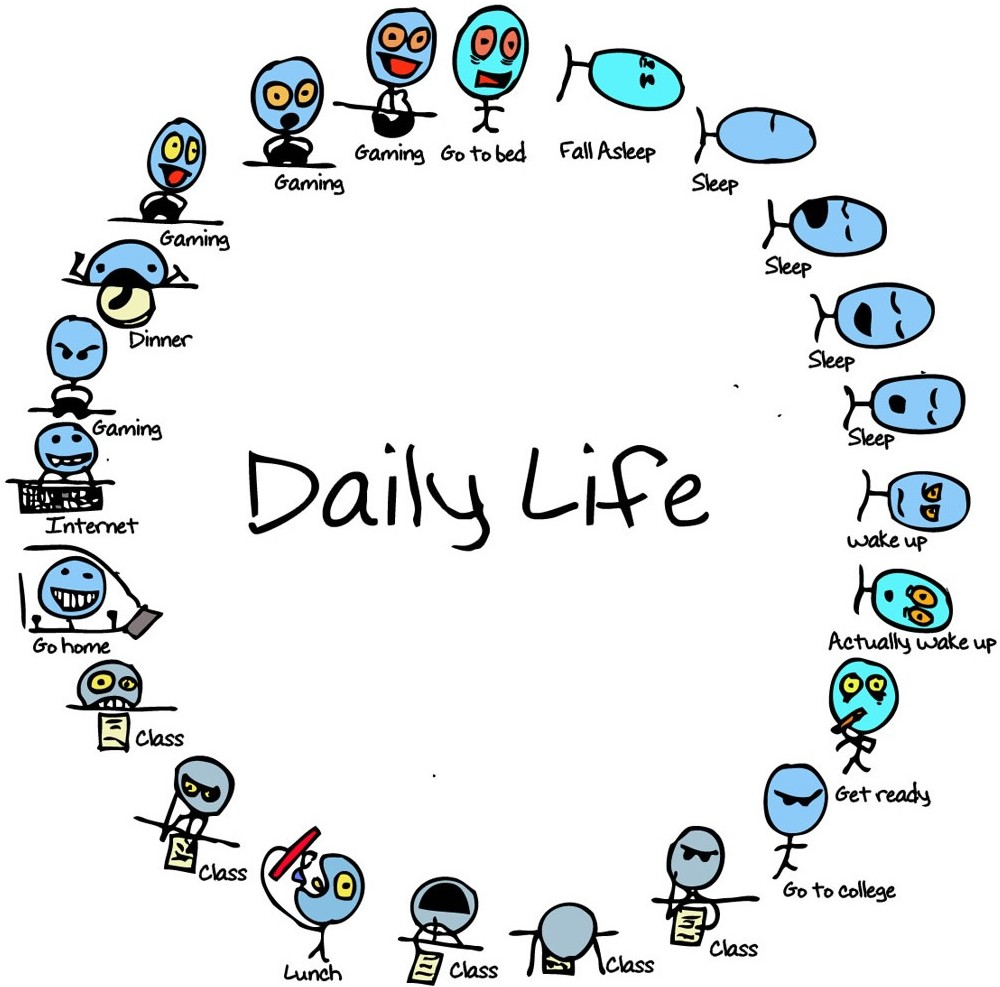
\includegraphics[width=0.37\textwidth]{c4_clock_01.jpg}
    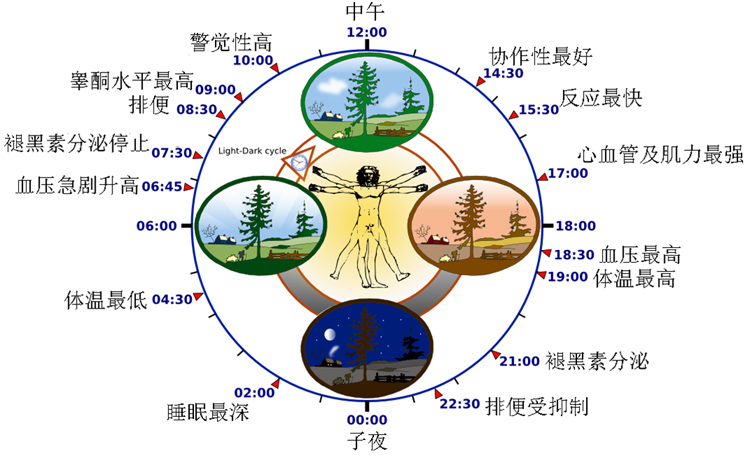
\includegraphics[width=0.61\textwidth]{c4_clock_03.jpg}
  \end{figure}
\end{frame}

% 1-8,1729
\begin{frame}
  \frametitle{生物钟 | 植物}
  \begin{block}{现象}
    \begin{itemize}
      \item 含羞草在夜间合拢叶片,白天打开。
      \item 如果把含羞草置于一个它无法知晓昼夜的环境中,情况会怎样呢?
    \end{itemize}
  \end{block}
  \pause
  \begin{block}{实验}
    \begin{itemize}
      \item 1729年,让\textbullet 雅克\textbullet 徳奥图斯\textbullet 德迈朗(天文学家)
      \item 把一株含羞草放到漆黑的柜中
    \end{itemize}
  \end{block}
  \pause
  \begin{block}{结果}
    \begin{itemize}
      \item 叶片在没有太阳光的情况下,还可以有规律地开合。
    \end{itemize}
  \end{block}
  \pause
  \begin{block}{启示}
    \begin{itemize}
      \item “时间生物学”(研究生物体内部的生物钟)的创立者
    \end{itemize}
  \end{block}
\end{frame}

% 1-109,1938
\begin{frame}
  \frametitle{生物钟 | 人}
  \begin{block}{疑问}
    人的睡眠规律究竟只是习惯,抑或是人体内存在着生物钟?
  \end{block}
  \pause
  \begin{block}{实验}
    \begin{itemize}
      \item 实验一:把生物钟从每天24小时调整为48小时、12小时——实验无果而终
      \item 实验二:把生物钟从每天24小时调整为21小时、28小时,测量体温——结果模棱两可
      \item 实验三:宽20米、高8米的猛犸洞窟(漆黑、安静、恒温)——结果显示出两面性
    \end{itemize}
  \end{block}
  \pause
  \begin{block}{启示}
随后的实验证实,\alert{人体内确实存在着生物钟}。它的运转大致跟一天24小时相吻合,并且每天都会根据实际时长进行自动调整。
  \end{block}
\end{frame}

% 2-128,1962
\begin{frame}
  \frametitle{生物钟 | 人}
  \begin{block}{穴居人——斯佛尔}
    \begin{itemize}
      \item 1962年,在洞穴里待2个月,不带钟表,观察自己的自然节律(每次起床、进食或者睡觉,都打电话通知值班人员,估算此刻的时间,值班人员记下真正的时间)
      \item 1972年,独自一人在德克萨斯州的“午夜”洞穴里度过了205天
      \item 1999年-2000年,在法国南部的克拉姆斯洞穴里生活了2个月
    \end{itemize}
  \end{block}
  \pause
  \begin{block}{结果}
    \begin{itemize}
      \item 斯佛尔在不知不觉中保持了早已习惯的24小时生活规律(睡8个小时,醒16个小时)。
      \item 每次起床后,误以为只经过短短几个小时便又去睡觉了,最终完全搞错了待在洞里的总体时间。
    \end{itemize}
  \end{block}
\end{frame}

\section{睡眠}
\begin{frame}
  \frametitle{睡眠}
  \begin{figure}
    \centering
    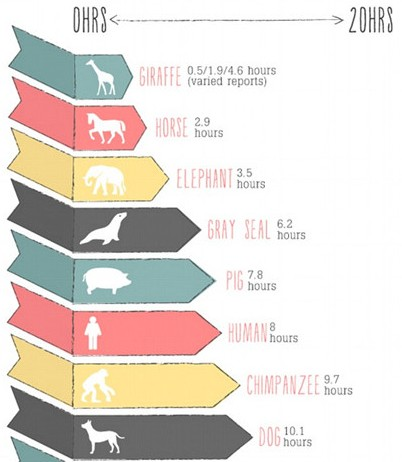
\includegraphics[width=0.45\textwidth]{c4_sleep_01.jpg}
    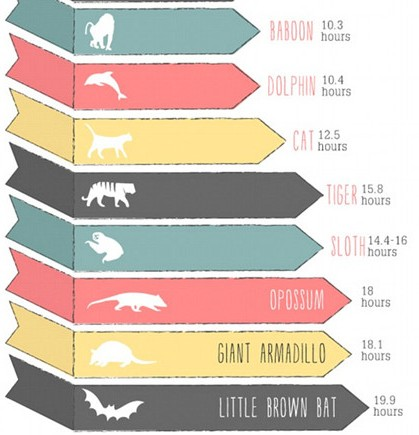
\includegraphics[width=0.45\textwidth]{c4_sleep_02.jpg}
  \end{figure}
\end{frame}

% 1-39,1894
\begin{frame}
  \frametitle{睡眠 | 狗}
  \begin{block}{疑问}
    \begin{itemize}
      \item 睡眠是一种不必要的习惯?
      \item 高等动物为何需要睡眠?(至今仍是未解之谜)
    \end{itemize}
  \end{block}
  \pause
  \begin{block}{实验(1894年)}
    \begin{itemize}
      \item 对4条幼犬实施睡眠剥夺:96~143小时之间死去
      \item 6条狗睡眠剥夺96~120小时之间时施救:死去
      \item 20~25天不进食:仍能自我恢复
    \end{itemize}
  \end{block}
  \pause
  \begin{block}{结论}
    “对动物而言,\alert{相比完全失去食物,彻底剥夺睡眠的结果更致命}”。
  \end{block}
\end{frame}

% 1-42,1895
\begin{frame}
  \frametitle{睡眠 | 人}
  \begin{block}{实验(1895年)}
    \begin{itemize}
      \item 3位男士,坚持90小时不睡觉
      \item 每6小时完成一项长达2小时的测试
    \end{itemize}
  \end{block}
  \pause
  \begin{block}{结果}
    \begin{itemize}
      \item 产生幻觉,无法电击醒,进入最深度的睡眠,……
      \item \alert{随着睡眠剥夺时间的增加,被试的注意力和记忆力明显消退。}
    \end{itemize}
  \end{block}
\end{frame}

% 2-137,1964
\begin{frame}
  \frametitle{睡眠 | 人}
  \begin{block}{缘起}
    1963年,参加学校举办的“科学博览会”——打破人类连续不眠的记录(260小时)。
  \end{block}
  \pause
  \begin{block}{疑问}
    极端的“睡眠剥夺”会对人体造成什么影响?
  \end{block}
  \pause
  \begin{block}{结果}
    \begin{itemize}
      \item 出现反应能力下降、注意力难以集中、视力障碍等症状。
      \item 在连续不眠264小时后,睡了14小时40分钟,身体就已基本恢复。
    \end{itemize}
  \end{block}
  \pause
  \begin{block}{启示}
    \begin{itemize}
      \item 进入《吉尼斯世界纪录》,后被多次打破,现已不再收录。
      \item 从不断刷新的不眠记录中并不能得到多少“睡眠剥夺”的知识。
    \end{itemize}
  \end{block}
\end{frame}

\section{饮食}
\begin{frame}
  \frametitle{饮食 | 素食 vs. 肉食}
  \begin{figure}
    \centering
    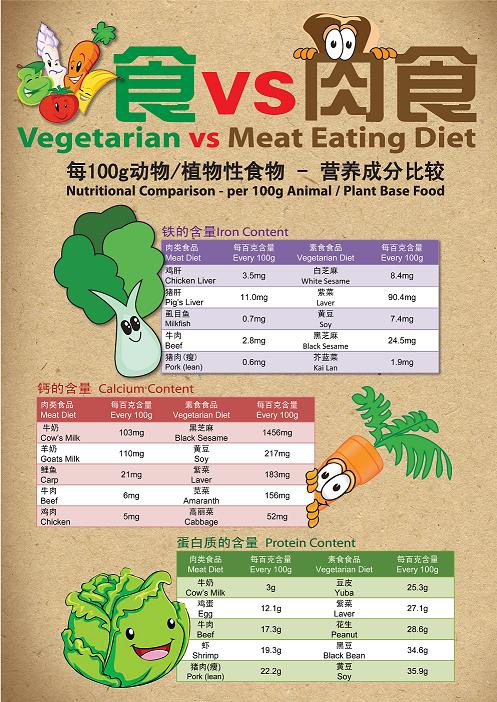
\includegraphics[width=0.8\textwidth]{c4_vm_01.jpg}
  \end{figure}
\end{frame}

% 2-55,1928
\begin{frame}
  \frametitle{饮食 | 肉}
  \begin{block}{疑问}
    怎么吃才健康?多吃蔬菜,少吃肉类?仅靠肉类能不能存活,健康会受到影响吗?
  \end{block}
  \pause
  \begin{block}{实验}
    \begin{itemize}
      \item 1913-1918:斯蒂芬森连续5年仅以肉类(鱼、北极熊、海豹和驯鹿)为食——过度食用肉类没有对其造成任何原本预计将会出现的有害影响。
      \item 1928,斯蒂芬森和安德森:常规饮食阶段(2周)——只吃肉(1年,斯蒂芬森只能吃瘦肉)——正常的“荤素搭配型”——实验末期(1周,安德森只能食用脂肪)
    \end{itemize}
  \end{block}
  \pause
  \begin{block}{结果}
    \begin{itemize}
      \item 斯蒂芬森和安德森终日食用肥腻食物,体重居然减轻了2千克。
      %\item 肉类食品含有的蛋白质并不像人们预想的那么丰富,脂肪才是它们富含的主要营养。(?)
    \end{itemize}
  \end{block}
\end{frame}

% 1-112,1945
\begin{frame}
  \frametitle{饮食 | 饥饿}
  \vspace{-0.5em}
  \begin{block}{疑问}
    饥饿会产生什么样的影响?
  \end{block}
  \vspace{-0.5em}
  \pause
  \begin{block}{实验}
    \begin{itemize}
      \item 36个拒服兵役的人,1944.11.19~1945.10.20
      \item 3个月的正常期——6个月的饥饿期——3个月的恢复期
      \item 正常期:检测健康状况、平均进食情况、新陈代谢的细节
      \item 饥饿期:每日2餐(早上8点半,下午5点),交替变换3份按照欧洲饥荒地区饮食制定的食谱(1500卡,此前的一半),按照被试各自的体重标准准确计算营养含量,在半年里使每个人减重1/4
      \item 恢复期:分成不同小组,按照不同的饮食计划重新恢复饮食
    \end{itemize}
  \end{block}
  \vspace{-0.5em}
  \pause
  \begin{block}{结果与启示}
    \begin{itemize}
      \item 《人类饥饿生物学》,身体与心理变化,影响智力、理解力及个性
      \item 对于研究消瘦病、进食障碍具有重要意义
    \end{itemize}
  \end{block}
\end{frame}

% 1-293,1999
\begin{frame}
  \frametitle{饮食 | 汤}
  \begin{block}{实验}
    招待3组女士餐前小吃——同样的配料,同样的热量:
    \begin{enumerate}
      \item 一个以鸡肉、米和蔬菜为原料的烤饼
      \item 烤饼加上356克水,混成浓汤状
      \item 烤饼,加上356克水
    \end{enumerate}
  \end{block}
  \pause
  \begin{block}{结果}
    \begin{itemize}
      \item 第二组在正餐时饭量足足减少了1/4
      \item 第二组使用的主菜量比第三组少了1/4
    \end{itemize}
  \end{block}
  \pause
  \begin{block}{启示}
    \begin{itemize}
      \item \alert{汤是馋鬼的敌人。}
      \item 科学在调节饥饿方面的认识是何等有限。
    \end{itemize}
  \end{block}
\end{frame}

\section{外部刺激}
% 1-137,1951
\begin{frame}
  \frametitle{外部刺激 | 隔音间}
  \begin{block}{疑问}
    \begin{itemize}
      \item 如果剥夺一切外界环境刺激,大脑会发生什么变化?
      \item 为什么\alert{从事单调工作的人在工作中容易出错}?
    \end{itemize}
  \end{block}
  \pause
  \begin{block}{实验}
22名被试,在一间隔音的、明亮的房间里躺在床上,手上戴着连指手套,前臂套着硬纸筒,双眼戴着仅能通过漫射光线的眼镜。
  \end{block}
  \pause
  \begin{block}{结果}
    \begin{itemize}
      \item 没人能在房间里坚持3天以上
      \item 隔绝严重损伤了思维能力:白日梦,注意力涣散
      \item 所有被试都产生了幻觉
    \end{itemize}
  \end{block}
\end{frame}

% 1-143,1955
\begin{frame}
  \frametitle{外部刺激 | 隔离箱 | 实验}
  \begin{block}{疑问}
    \begin{itemize}
      \item 如何加强与外界的隔绝从而急剧加强幻觉?
      \item 当一切外界刺激都被阻断后,人脑会有何反应?
    \end{itemize}
  \end{block}
  \pause
  \begin{block}{猜测}
    \begin{enumerate}
      \item 大脑进入休眠,人体失去意识,进入昏迷状态。
      \item 大脑仍然活动,通过内部的调节机制保持清醒。
    \end{enumerate}
  \end{block}
  \pause
  \begin{block}{实验}
      在隔离箱(放置在隔除噪音的漆黑房间内,充满34.5摄氏度的温水,安装有舒适的呼吸面具,水定时更新)中生活一年
  \end{block}
\end{frame}

\begin{frame}
  \frametitle{外部刺激 | 隔离箱 | 结果}
  \begin{block}{结果}
(前3刻钟)浮现生活琐事,非常清醒地知道自己在哪儿——(3刻钟后)开始放松,告诉自己什么都不用做——(一小时后)渴望来自外部的刺激——浮想联翩——出现幻觉
  \end{block}
  \pause
  \begin{block}{结论与结局}
    \begin{itemize}
      \item 大脑在缺乏外部刺激时,不会陷入休眠状态,完全相反,我们的大脑似乎很懂得自娱自乐。
      \item 家用隔离箱(Samadhi箱),精神病学(精神分裂症),洗脑,心灵传递 $\rightarrow$人类心灵的新理论 $\rightarrow$ 秘传运动领导人
    \end{itemize}
  \end{block}
\end{frame}

\section{蜘蛛实验}
% 1-125,1948
\begin{frame}
  \frametitle{蜘蛛实验 | 药物}
  \begin{block}{缘起}
    \begin{itemize}
      \item 希望拍摄蜘蛛织网的过程,但它们总是在凌晨4点钟的时候织网。
      \item 能否使用兴奋剂,控制蜘蛛在合适的时间织网。
    \end{itemize}
  \end{block}
  \pause
  \begin{block}{结果}
    结果未遂人愿!但蜘蛛在药物影响下织出的网却是见所未见的。
  \end{block}
  \pause
  \begin{block}{灵感}
    能否通过蛛网来量化药物作用的效果? $\Longrightarrow$ 量化药物对有机体的影响!
  \end{block}
  \pause
  \begin{block}{结局}
    \begin{itemize}
      \item 把蛛网作为一种通行的化学药物指示剂的希望落空了。
      \item 不再关注对使用的药物的识别,而是特定药物对蜘蛛神经系统的影响。
    \end{itemize}
  \end{block}
\end{frame}

% 1-142,1955
\begin{frame}
  \frametitle{蜘蛛实验 | 尿液}
  \vspace{-0.5em}
  \begin{block}{缘起}
    蜘蛛在药物作用下织出异常蛛网 $\Rightarrow$ 利用蜘蛛解开精神分裂症的秘密
  \end{block}
  \vspace{-0.5em}
  \pause
  \begin{block}{已知与疑问}
    \begin{itemize}
      \item 正常人摄入一定量的莫斯卡灵和LSD后,会出现跟精神分裂症病人类似的症状(幻觉和精神错乱)。
      \item 精神分裂症病人的新陈代谢是否会持续不断地产生这种化学物质?
      \item 是否是这种化学物质导致他们情绪持续亢奋?
    \end{itemize}
  \end{block}
  \vspace{-0.5em}
  \pause
  \begin{block}{实验与结果}
    \begin{itemize}
      \item 15位精神分裂症病人,50升尿液,浓缩处理,喂食蜘蛛,将其所织的蛛网对比喂食正常尿液的蜘蛛织出的蛛网,进行分析。
      \item 2组喂食不同尿液浓缩物的蜘蛛织出的蛛网确有不同,但是这些区别中并无任何规律。
      \item 蛛网不同的几何构造对精神分裂症的病因调查无任何借鉴意义。
    \end{itemize}
  \end{block}
\end{frame}

% 1-139,1952
\begin{frame}
  \frametitle{蜘蛛实验 | 断腿}
  \begin{block}{缘起}
    还在为孩童时期揪下过蜘蛛腿而至今心存不安?
  \end{block}
  \pause
  \begin{block}{实验}
    \begin{itemize}
      \item 最多截去蜘蛛的2条腿:一左一右
      \item 用电影摄像机监视织网情况
      \item 约10000次个案研究,48页研究报告
    \end{itemize}
  \end{block}
  \pause
  \begin{block}{结果}
    “在失去一条或者几条腿后,蜘蛛仍旧能够按照既定目标完成织网。”
  \end{block}
\end{frame}

% 1-246,1973
\begin{frame}
  \frametitle{蜘蛛实验 | 失重}
  \begin{block}{疑问}
    在失重状态下蜘蛛织出的蛛网是什么样子的?
  \end{block}
  \pause
  \begin{block}{实验}
    1973年7月28日,2只十字蜘蛛,Apollo-Kapsel号,美国的天工空间站
  \end{block}
  \pause
  \begin{block}{结论}
    蜘蛛可以适应失重环境并在这种不寻常的状态下织出正常的蛛网。
  \end{block}
  \pause
  \begin{block}{启示}
   从蜘蛛在宇宙中的作品中发现了一种新的网球拍设计原则——“火箭网球拍”。
  \end{block}
\end{frame}

\section{狗}
% 1-294,2002
\begin{frame}
  \frametitle{狗 | 最优问题}
  \begin{block}{问题}
    \begin{itemize}
      \item 什么时候从岸上跳入水中开始游泳?(游泳比奔跑要慢)
      \item 什么时候从一条没有雪的路转向有雪的路?
    \end{itemize}
  \end{block}
  \vspace{-0.3em}
  \pause
  \begin{block}{策略}
    \begin{enumerate}
      \item 立刻跳入水中,直接游向网球——最短的路,但不是最快的
      \item 沿着河岸跑,直到球和它呈垂直角度时跳进水中——游的距离最短,总路程最长
      \item 起初沿着河岸跑一段,然后斜着向球游去——最快的捷径
    \end{enumerate}
  \end{block}
  \vspace{-0.3em}
  \pause
  \begin{block}{狗能否解决这一优化问题?}
    \begin{itemize}
      \item 把球扔到水里,狗去捡,重复了40多次
      \item 计算狗在岸上和水中的速度,计算出理想的入水处
      \item 狗几乎每次都(凭直觉)选择了正确的位置。
    \end{itemize}
  \end{block}
\end{frame}

\begin{frame}
  \frametitle{狗 | 最优问题}
  \begin{block}{\alert{最小作用量原理}}
    \begin{figure}
      \centering
      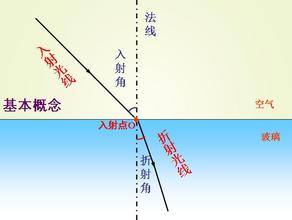
\includegraphics[width=0.3\textwidth]{c4_lap_01.jpg} \ 
      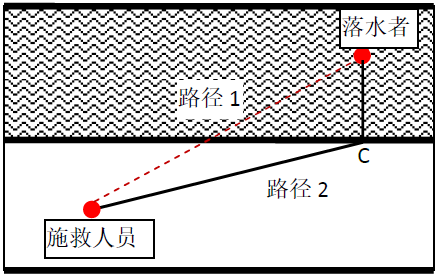
\includegraphics[width=0.36\textwidth]{c4_lap_02.png} \ 
      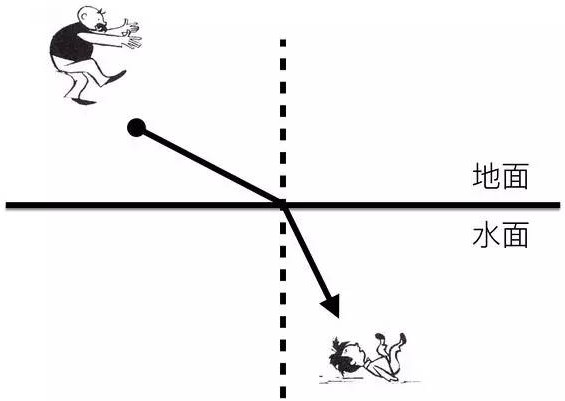
\includegraphics[width=0.32\textwidth]{c4_lap_03.jpg}
    \end{figure}
  \end{block}
\end{frame}

% 1-296,2003
\begin{frame}
  \frametitle{狗 | 机器狗}
  \begin{block}{疑问}
    \begin{itemize}
      \item 动物狗是否会把机器狗当成自己的同类?
      \item 用廉价的仿真模型来迷惑动物?
    \end{itemize}
  \end{block}
  \vspace{-0.5em}
  \pause
  \begin{block}{实验}
    \begin{itemize}
      \item 把40条狗和一条身长30厘米、重1.5公斤的机器狗(有时穿上前一天放到幼犬睡篮中的皮毛)关在一起,观察它们的行为。
      \item 测试狗和真正的幼犬以及车模在一起的行为。
      \item 研究狗对机器狗的关注程度、两者间的距离,以及狗对机器狗吠叫、咆哮和嗅闻(前面和后面)的次数。
    \end{itemize}
  \end{block}
  \vspace{-0.5em}
  \pause
  \begin{block}{结果与结论}
    \begin{itemize}
      \item 狗虽然对机器狗有反应,程度上却显然要弱于面对幼犬。
      \item 对于把机器狗应用于狗行为的研究中,尚存在一些重大的局限。
    \end{itemize}
  \end{block}
\end{frame}

% 2-284,2006
\begin{frame}
  \frametitle{狗 | 助人为乐}
  \begin{block}{目的}
    通过一项实验来科学地研究犬类助人为乐的特性。
  \end{block}
  \pause
  \begin{block}{实验}
    \begin{itemize}
      \item 44条狗,15个种类
      \item 2个情景:一个是主人假装心肌梗死,另一个是主人被翻到的架子压住。
    \end{itemize}
  \end{block}
  \pause
  \begin{block}{结果}
    几乎没有一条狗去寻求帮助、救助主人!
  \end{block}
  \pause
  \begin{block}{启示}
    \begin{itemize}
      \item 实验情景缺乏戏剧性,不够紧张刺激。(没有生成气味信息素)
      \item 在驯化过程中,狗逐渐丧失了独立应对外部世界的能力、空间记忆。
    \end{itemize}
  \end{block}
\end{frame}

% 2-291,2007
\begin{frame}
  \frametitle{狗 | 不对称性}
  \begin{block}{已知}
    \begin{itemize}
      \item 大脑的不对称性导致了人类和其他灵长类动物更加偏好使用右手。
      \item 右脑控制身体左侧,左脑控制身体右侧。
      \item 大脑的两半部分负责不同的情绪:左脑一般负责亲近和信任,右脑则专门负责逃避、不信任、恐惧、抑郁。具体表现为:人类面部右侧的肌肉反映愉悦和满足,左侧的肌肉则反映悲伤和不满。
      \item 狗用尾巴表达自己的情绪状态。
    \end{itemize}
  \end{block}
  \pause
  \begin{block}{疑问}
    不对称性是如何在非成对出现的身体部位(狗的尾巴)中发挥作用的?
  \end{block}
\end{frame}

\begin{frame}
  \frametitle{狗 | 不对称性}
  \begin{block}{实验}
    \begin{itemize}
      \item 30条狗,2米 X 2米 X 4米的暗箱
      \item 狗进入暗箱,通过窗口依次看到猫、更强势的狗、陌生人或者主人
      \item 摄像机从上向下拍摄,记录它们的尾巴是怎样摇摆的
    \end{itemize}
  \end{block}
  \vspace{-0.5em}
  \pause
  \begin{block}{结果}
    \begin{itemize}
      \item 狗看到主人时,摇尾巴就会更加偏向右边,见到陌生人和猫的时候也有向右偏的倾向。
      \item 当狗面对一条更加强势的狗时,摇尾巴就会更加偏向左边。
      \item 一切让狗感觉受到“吸引”的外界刺激都会使狗向右摇尾巴。如果狗准备逃跑,就会向左摇尾巴。
    \end{itemize}
  \end{block}
  \vspace{-0.5em}
  \pause
  \begin{block}{启示}
    为什么大脑的构造是不对称的? $\Longrightarrow$ 语言?同时做2件事?内脏?
  \end{block}
\end{frame}

% 2-294,2008
\begin{frame}
  \frametitle{狗 | 打哈欠}
  \begin{block}{已知}
    打哈欠并不是由缺氧引起的,可以冷却大脑,会传染。
  \end{block}
  \pause
  \begin{block}{猜测}
    \begin{itemize}
      \item 打哈欠也许具有社会功能。
      \item 打哈欠之所以能够发挥传染效应,是因为人们具有体谅他人的能力。
    \end{itemize}
  \end{block}
  \pause
  \begin{block}{实验——自闭症患者}
    自闭症患者认识不到“他人和自己一样”!
    \begin{itemize}
      \item 49名儿童(24名自闭症患儿),录像中含有6张打哈欠的脸
      \item 自闭症患儿打哈欠的次数确实更少,是其他儿童的1/3。
    \end{itemize}
  \end{block}
\end{frame}

\begin{frame}
  \frametitle{狗 | 打哈欠}
  \begin{block}{实验——狗}
    要做到“体谅他人”,需要进行复杂的思考,还要拥有认识自我的能力。这2点都是狗所不具备的。
    \begin{itemize}
      \item 29条狗,助手在狗朝他看的时候,在接下来的5分钟内打10~20个哈欠
      \item 29条狗中有21条跟着打起了哈欠,平均发生在1分39秒之后
      \item 模仿张嘴的动作,反复张开又闭上嘴巴但不是打哈欠,狗没有出现任何反应
    \end{itemize}
  \end{block}
  \pause
  \begin{block}{启示}
    \begin{itemize}
      \item 从人类传染到狗,打哈欠的传染效应成功跨越了物种界限。
      \item 受到传染而打哈欠的狗的比例非常高:72\%(人与人45\%~50\%,人与黑猩猩33\%)。
      \item 可能意味着,\alert{狗对人类的理解比人与人之间的理解更加深入}。
    \end{itemize}
  \end{block}
\end{frame}

\section{史海撷华}
% 1-6,1620
\begin{frame}
  \frametitle{史海撷华 | 光合作用}
  \begin{block}{种柳行动}
    \begin{itemize}
      \item 范\textbullet 黑尔蒙特(最后一个炼金术士,第一个化学家),首位用泥土、树木和称实际操作实验的人
      \item 200磅在炉中烘干的泥,5磅重的柳树幼枝,定期浇水
      \item 5年后拔出柳树,对土和柳树分别称重
    \end{itemize}
  \end{block}
  \vspace{-0.75em}
  \pause
  \begin{block}{结果与结论}
    \begin{itemize}
      \item 泥土减重2盎司,树木增重164磅零3盎司
      \item 164磅的木质、树皮以及根系都只来源于水(当时唯一合理的结论)
    \end{itemize}
  \end{block}
  \vspace{-0.75em}
  \pause
  \begin{block}{启示}
    \begin{itemize}
      \item 为\alert{实验}铺平了道路,使其从此成为\alert{获取认识的手段}
      \item 他的想法启发了很多的学者,开展罐中植物的研究
      \item 为“光合作用”这一神秘过程的探究开了先河
      \item 学生借此测试洞察力,练习严谨的实验设计
    \end{itemize}
  \end{block}
\end{frame}

% 1-12,1774
\begin{frame}
  \frametitle{史海撷华 | 温度耐受}
  \begin{block}{疑问}
    人体能够承受什么样的温度?
  \end{block}
  \pause
  \begin{block}{实验}
    \begin{itemize}
      \item 建造桑拿室,45$^{\circ}$C-100$^{\circ}$C-127$^{\circ}$C
      \item 穿衣服发汗,赤裸着手持一只平底锅,上面放着一块牛排
    \end{itemize}
  \end{block}
  \pause
  \begin{block}{结果及结论}
    \begin{itemize}
      \item 24页的《皇家协会学报》
      \item 有一个“与生命体直接相关的自然的系统”消除热量?(降温——汗液等的蒸发加之以血液流动!)
    \end{itemize}
  \end{block}
\end{frame}

% 1-16,1802
\begin{frame}
  \frametitle{史海撷华 | 蛙腿实验}
  \begin{block}{现象}
    如果用两种不同的金属触碰蛙腿,连成通路,它们的肌肉会抽搐。
  \end{block}
  \pause
  \begin{block}{观点}
    \begin{itemize}
      \item 加尔瓦尼:“动物电流”与生命力有关,效果与电流通过无生命的物质是不同的。
      \item 伏特:世界上只有一种电,无论是雷雨天的闪电还是抽搐的蛙腿,原理都与这种电有关。
    \end{itemize}
  \end{block}
  \pause
  \begin{block}{启示}
    \begin{itemize}
      \item 《弗兰肯斯坦》(第一部科幻小说)——玛丽\textbullet 雪莱
      \item 眨眼睛的尸体——对于绞死者进行头颅实验
    \end{itemize}
  \end{block}
\end{frame}

% 1-140,1954
\begin{frame}
  \frametitle{史海撷华 | “弗兰肯斯坦”}
  \begin{figure}
    \centering
    
\includegraphics[width=0.46\textwidth]{c4_frankenstein_01.jpg}\quad
    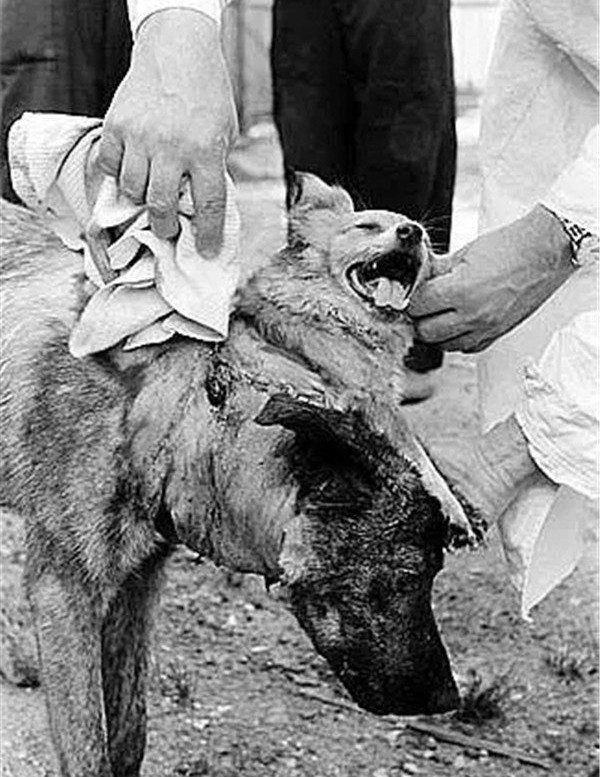
\includegraphics[width=0.46\textwidth]{c4_frankenstein_02.jpg}
  \end{figure}
\end{frame}

% 1-20,1825
\begin{frame}
  \frametitle{史海撷华 | 胃上有洞的人}
  \begin{block}{实验材料}
       1882年,威廉\textbullet 博蒙特;亚力克西斯\textbullet 圣马丁(受伤的士兵)
  \end{block}
  \vspace{-0.5em}
  \pause
  \begin{block}{疑问}
消化仅仅是一个纯化学的过程,还是同时需要人体提供某种未知的生命力量促使其完成?消化和腐烂的区别是否在于前者拥有人体内的未知生命力量,而后者没有?
  \end{block}
  \vspace{-0.5em}
  \pause
  \begin{block}{实验}
      用丝线系好的食物,塞入胃中——拉出,观察消化情况;插入软管、导出胃液,把一把牛肉粒置于其中;……
  \end{block}
  \vspace{-0.5em}
  \pause
  \begin{block}{结果}
    \begin{itemize}
      \item 器皿中胃液的化学能量足以完成消化(无需未知的生命力量)。
      \item 推翻了胃液仅仅是流于胃中储存起来的唾液的推测。
      \item 医学伦理
    \end{itemize}
  \end{block}
\end{frame}

% 1-59,1902
\begin{frame}
  \frametitle{史海撷华 | 条件反射}
  \begin{block}{现象}
    \begin{itemize}
      \item 研究初衷:给狗提供不同食物的时候,狗分泌的消化液的构成。
      \item 出现问题:作为实验对象的狗被喂过几次之后,仅仅看见喂它的人就开始分泌唾液。
      \item 改进实验:不给任何提示就直接将食物送进狗的口中,问题依旧!
      \item 巴甫洛夫:干扰因素、实验的缺陷? $\Longrightarrow$ 一个全新的研究领域!
    \end{itemize}
  \end{block}
  \vspace{-0.5em}
  \pause
  \begin{block}{实验}
    \begin{itemize}
      \item 在给狗提供食物之前给出特定的信号(铃铛、节拍器、电子钟)
      \item 在隔音房中,借助操纵杆和滑轮进行实验而不对实验对象产生干扰
    \end{itemize}
  \end{block}
  \vspace{-0.5em}
  \pause
  \begin{block}{启示}
    \begin{itemize}
      \item 经典条件反射学说 $\Longrightarrow$ 学习的基本程序
      \item 如何让已经存在的条件反射消失 $\Longrightarrow$ 行为治疗学
    \end{itemize}
  \end{block}
\end{frame}

% 1-89,1927
\begin{frame}
  \frametitle{史海撷华 | 亲吻培养基}
  \begin{block}{舆论}
    梅毒患者每次接吻所传播的病菌数量达到40000 $\Longrightarrow$ “反接吻联盟”
  \end{block}
  \pause
  \begin{block}{实验}
    \begin{itemize}
      \item 几位先生和女士,亲吻无菌培养基,在摄氏37.5度的保温箱中放置24小时
      \item 亲吻时黏附的细菌生成菌落,计算得出细菌数量
    \end{itemize}
  \end{block}
  \pause
  \begin{block}{结果与结论}
    \begin{itemize}
      \item 细菌平均数量为500,涂抹口红的女士携带的细菌要多200
      \item 拒绝亲吻化妆后的嘴唇!
    \end{itemize}
  \end{block}
\end{frame}

% 1-179,1962 
\begin{frame}
  \frametitle{史海撷华 | 致幻剂}
  \vspace{-0.5em}
  \begin{block}{疑问}
    致幻剂是否能够使人产生类似极少数人在宗教狂热中所感受的神秘感觉?
  \end{block}
  \vspace{-0.5em}
  \pause
  \begin{block}{实验}
    \begin{itemize}
      \item 双盲实验,4人一组(2人陪同),4颗胶囊(2颗致幻剂+2颗安慰剂)
      \item 问卷调查、回答问题(2个半小时后,第二天,6个月后,25年后)
    \end{itemize}
  \end{block}
  \vspace{-0.5em}
  \pause
  \begin{block}{结果}
    \begin{itemize}
      \item 10名服用致幻剂的学生中,有8人体验到至少7种神秘和超验的感觉和感受。
      \item 对照组中没有人达到该程度(在所有项目上他们都落后于实验组)。
      \item \alert{实验的经历对于他们(实验组)的日常生活产生了积极的效果。}
      \item 25年后(16/19/20人),实验组和对照组都给出了和1/4世纪前相似的回答。
    \end{itemize}
  \end{block}
\end{frame}

% 1-184,1962
\begin{frame}
  \frametitle{史海撷华 | 触觉}
  \begin{block}{饼干模子实验}
    \begin{enumerate}
      \item 压在手心(49\%) vs. 拿在手里触摸(95\%)
      \item 按在手心,保持静止或以微小的频率转动(49\%) vs. 在模子移动的情形下用指尖感知形状(72\%)
    \end{enumerate}
  \end{block}
  \pause
  \begin{block}{结论}
    \begin{itemize}
      \item 最可靠最便捷的感知某种形状的方法,显然是用手指触摸它。
      \item “\alert{皮肤对物体形状的感知越是不清晰,大脑对它的感知则越清晰。}”
      \item 触觉并非是神经对外界刺激的被动反应和消极传递过程。触觉对形状做着主动搜索,产生对外界刺激的反射生物电流。大脑随时准备对不停变化的触觉信号做出筛选,从以前的生活经历中,寻找一个相匹配的固定形状。
    \end{itemize}
  \end{block}
\end{frame}

% 2-143,1966 
\begin{frame}
  \frametitle{史海撷华 | 小岛生物地理学}
  \begin{block}{理论}
    \begin{itemize}
      \item 一定面积的小岛能够容纳的物种数是有上限的(标准定额)。
      \item 标准定额取决于两个因素:小岛的面积以及小岛与大陆之间的距离。
      \item 有新物种迁入,也有老物种消失——动态平衡。
    \end{itemize}
  \end{block}
  \pause
  \begin{block}{实验}
    把岛上的昆虫消灭干净:喷洒杀虫剂 $\Longrightarrow$ 包装小岛、毒气熏蒸
  \end{block}
  \pause
  \begin{block}{启示}
    \begin{itemize}
      \item 它将一种描述性的科学变成了实验性的科学。
      \item 实验的结果不仅适用于小岛。(指导建立自然保护区)
      \item SLOSS(单个大面积还是多个小面积)?——至今还没找到明确答案!
    \end{itemize}
  \end{block}
\end{frame}

% 2-189,1986 
\begin{frame}
  \frametitle{史海撷华 | 经期同步化}
  \begin{block}{现象}
    每次吉纳维夫\textbullet 斯维茨与别的女性同住,几个月后,她们都会和她同时来月经。
  \end{block}
  \pause
  \begin{block}{已知}
    女性之间关系密切,月经周期往往趋于同步。(调查宿舍楼里135名女同学,亲密朋友:暑假刚结束时相差6天半,7个月后相差4天半)
  \end{block}
  \pause
  \begin{block}{实验}
      将药棉球夹在腋下,收集汗液;在实验组上唇部位涂抹(对照组使用只含酒精的棉球)
  \end{block}
  \pause
  \begin{block}{结果}
      4个月后,5名实验组女性的月经周期差距缩短,仅为3-4天,比研究开始时少了6天。对照组6名女性的周期并未出现同步趋势。
  \end{block}
  % \pause
  % \begin{block}{启示}
  %   时至今日,仍有许多专业认识质疑“经期同步化”现象是否真的存在。人们后来针对这一问题研究了各种女性群体,始终没有得出明确结论。
  % \end{block}
\end{frame}

% 2-245,1996 
\begin{frame}
  \frametitle{史海撷华 | 站 vs. 坐(vs. 躺)}
  \begin{figure}
    \centering
    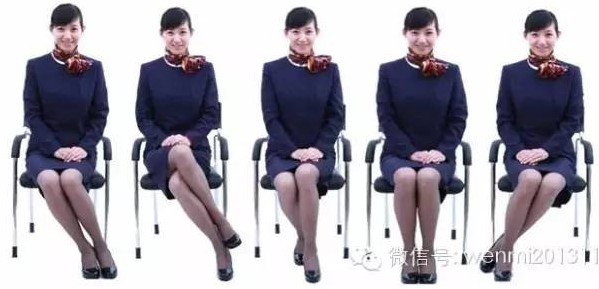
\includegraphics[width=0.65\textwidth]{c4_sit_01.jpg}\\
    
\includegraphics[width=0.6\textwidth]{c4_sit_05.jpg}
  \end{figure}
\end{frame}

\begin{frame}
  \frametitle{史海撷华 | 站 vs. 坐(vs. 躺)}
  \begin{block}{“背部学说”}
    \begin{itemize}
      \item 坐直比懒洋洋地靠着要好。
      \item 坐姿时的压力几乎是站姿时的一倍半。
      \item 坐着的时候模仿站姿、挺直背部(“女秘书坐姿”),具有保护背部的作用。
    \end{itemize}
  \end{block}
  \vspace{-0.5em}
  \pause
  \begin{block}{实验}
    背部植入探针压力计。
  \end{block}
  \vspace{-0.5em}
  \pause
  \begin{block}{结果}
    \begin{itemize}
      \item 平躺时背部受到的压力最小,放松站立时压力提高5倍。
      \item 站姿和坐姿的压力大致处在一个范围,并无明显区别。
      \item 采用半躺半坐的体位(“葛优躺”?)时,压力达到最小。
      \item \alert{重要的不是保持“正确”的姿势,而是时常改变坐姿。}
    \end{itemize}
  \end{block}
\end{frame}

% 2-260,2001
\begin{frame}
  \frametitle{史海撷华 | 迷宫中的精子}
  \begin{block}{疑问}
    把老鼠送进迷宫可以研究它们的记忆,换成精子呢?
  \end{block}
  \pause
  \begin{block}{实验}
    \begin{itemize}
      \item T字形迷宫:714个精子中有351个(49\%)游向了左边,有363个(51\%)游向了右边。
      \item 直角状的入口(先右转)+ T字形迷宫:588个精子更多地(59\%)转向左边。
    \end{itemize}
  \end{block}
  \pause
  \begin{block}{启示}
    \begin{itemize}
      \item 精子以某种方式成功地存储了“刚刚走过右边”这一信息。
      \item 人们放进迷宫的每一种有机体都做出过这种行为。
      \item 科学研究将这种改换方向的行为称为“自发性更迭行为”。
      \item 人们推测,在觅食和勘察领地的过程中,这种走法更加利于存活。
    \end{itemize}
  \end{block}
\end{frame}

% 2-289,2006
\begin{frame}
  \frametitle{史海撷华 | 立体嗅闻}
  \begin{block}{现象}
  器官成对出现:有2只眼睛看到的东西才是立体的,有2只耳朵才能给声音定位。
  \end{block}
  \pause
  \begin{block}{疑问}
    \begin{itemize}
      \item 为什么人和动物都有2个鼻孔呢?(猜想:2个鼻孔能够帮助动物实现定向嗅闻。——难以置信,难以验证!)
      \item 2个鼻孔会比1个鼻孔让人更快追踪到某种气味的痕迹吗?
      \item 人类到底能不能够追踪气体的痕迹?
    \end{itemize}
  \end{block}
  \pause
  \begin{block}{实验}
    在草坪中埋下曾在高度稀释的巧克力溶液中浸泡过的打包绳,32名被试者,蒙住眼睛,在距离巧克力痕迹3米远的地方跪下并开始嗅闻。
  \end{block}
\end{frame}

\begin{frame}
  \frametitle{史海撷华 | 立体嗅闻}
  \begin{block}{结果}
    \begin{itemize}
      \item 2/3的被试者能够发现踪迹,一路追寻巧克力的香气,直到终点。
      \item 封住1只鼻孔的14名被试者仍然可以抵达目的地的比例变成了1/3,速度比之前要慢很多。
    \end{itemize}
  \end{block}
  \vspace{-0.6em}
  \pause
  \begin{block}{猜测}
     导致效能变差的原因:
     \begin{enumerate}
       \item 方向信息缺乏
       \item 吸入的气味分子数量减半、只接触半数感觉细胞
     \end{enumerate}
  \end{block}
  \vspace{-0.6em}
  \pause
  \begin{block}{实验}
    \begin{itemize}
      \item 使用配件(1个鼻孔吸入空气但分布到2个鼻孔中),成功率仍然比最初测试时低,速度也很缓慢。
      \item 之前的实验中确实运用了立体嗅闻的能力。
      \item 通过使嗅闻频率翻倍可以提高追踪效率。
    \end{itemize}
  \end{block}
\end{frame}

\begin{frame}
  \frametitle{史海撷华 | 借酒消愁}
  \vspace{-0.5em}
  \begin{block}{疑问}
    \begin{itemize}
      \item 已知:当果蝇饮用酒精时,大脑内的奖赏通路即被激发,它们就会有“心情愉悦”的感觉。社交互动是最有奖赏效应的经历之一。
      \item 疑问:这两种类型的奖赏是否会在脑部发生联系?
  \vspace{-0.2em}
    \end{itemize}
  \end{block}
  \vspace{-0.6em}
  \pause
  \begin{block}{实验}
    \begin{itemize}
      \item 24只雄性果蝇,随机分成2组
        \begin{itemize}
          \item 可以和多个雌性果蝇交配:按4只一小组放入3支小玻璃瓶中,每支小玻璃瓶内有20只等待交配的雌性果蝇
          \item 单独放在小玻璃瓶中,每个瓶内只有一只已经交配过的雌性果蝇(由于已经交配过,所以会排斥任何求爱的行为)
        \end{itemize}
  \vspace{-0.5em}
      \item 4天的反复交配和反复被拒后,移到新的容器中(分别装有添加酒精和不含酒精的糊状的食物),测量果蝇的进食量
  \vspace{-0.2em}
    \end{itemize}
  \end{block}
  \vspace{-0.6em}
  \pause
  \begin{block}{结果——《\textit{Science}》}
    \begin{itemize}
      \item 求爱被拒的果蝇饮用的酒精量要比成功交配的果蝇多4倍
      \item 被拒的雄性果蝇,脑部的神经肽F(NPF)仅有成功交配的一半
      % \item 包括人类在内的哺乳动物有一种类似神经肽F的蛋白质——神经肽Y
  \vspace{-0.2em}
    \end{itemize}
  \end{block}
\end{frame}

\begin{frame}
  \frametitle{史海撷华 | 其他}
  \begin{block}{真正的疯狂}
    \begin{itemize}
      % 1-24,1837
      \item 蚯蚓没有听觉——达尔文为蚯蚓演奏巴松管、笛子和钢琴
      % 1-29,1852
      % “迪谢纳肌营养不良症”
      \item 科学 vs. 艺术——破译人类面部表情,真心的笑 vs. 虚伪的笑
      % 1-40,1894
      \item 下落的猫咪——每秒完成60次成像的连拍胶片照相机
      % 1-43,1896
      \item 视网膜成像——颠倒的世界,对比参照其他元素、和谐化处理
      % 1-55,1901
      \item 灵魂重21克——6个人(结核病人),15条狗(毒死?)
      % 1-188,1963
      \item 遥控斗牛(大脑的电击刺激)——知识本身并没有错,如何去应用知识,结果会有不同!
      % 1-285,1992
      \item 核磁共振仪下的“飞去来器”——获得搞笑诺贝尔奖
      % 2-158,1968
      \item \alert{枪打出头鸟}——用颜色标记的牛羚一定会在下一次袭击时遭到猎杀
      % 2-165,1970
      \item 1头海豚 vs. 40名裸女——海豚为何能够在水中高速游动?
      % 2-177,1977
      \item “完美的钟摆”——非洲女性的完美行走方式
      % 2-205,1991
      \item “生物圈2号”——温室 $\Longrightarrow$ 地球 $\Longrightarrow$ 宇宙
    \end{itemize}
  \end{block}
\end{frame}



\section*{Acknowledgements}
\begin{frame}
  \frametitle{Powered by}
  \begin{center}
    
\includegraphics[width=9cm]{power.png}
  \end{center}
\end{frame}

\end{document}

